\chapter{Engineering model}
\label{Engineering_model_chapter}
This chapter will describe engineering model developed during this thesis.

This model should be as close to flight model as possible - but it could be e.g. on separate board, which is this case.

This model was developed as flight-ready version for sensor calibration \& tests along with developing \& testing flight software.

\section{Background - calibration stand}
    During development of the system previous model was developed to test and calibrate MOSFET transistors to use as a radiation dosimeters. Calibration stand was developed by M. Gumiela in his engineering thesis \cite{MGThesis}. The basic goal was to develop measurement device which can be used to determine final operational point, calibrate radiation response and to perform temperature calibration of flight sensor.

    The test and calibration stand allows to carry out simultatenous investigation of parameters of multiple MOSFETs (i.e. 18) and diodes (i.e. 6). It is possible to obtaing transfer characteristics of the DUT (I-V) utilizing adjustable constant current source, thermal calibration (Vth(T), Vd(T)) thanks to precise reference thermometers, Iztc investigation and finally TID on-line calibration.


\section{Block diagram}
    Block diagram of proposed system based on CD4007 is presented in the figure \ref{sensor_block_diagram}.

    It was designed having in mind miniaturization of sensor - to fit on PW-Sat2 PLD board. Because CD4007 has 3 complementary MOS pairs it was proposed to use 3 p-MOS transistors as TID sensors - to improve fidelity of the measurements. One n-MOS is used as a temperature sensor. Current source and ADC are multiplexed between 4 channels - this reduces board footprint and increases sensor reliability \& accuracy. Having in mind readout fidelity 3-wire method on multiplexer was implemented.

    System consists of few basic building blocks, each of them will be detailed in this chapter:
    \begin{itemize}
        \item \SI{125}{\uA} constant current source,
        \item CD4007 sensing element (3x p-MOS \& 1x n-MOS),
        \item differential ADC,
        \item multiplexer
    \end{itemize}


    \begin{figure}[H]
        \centering
        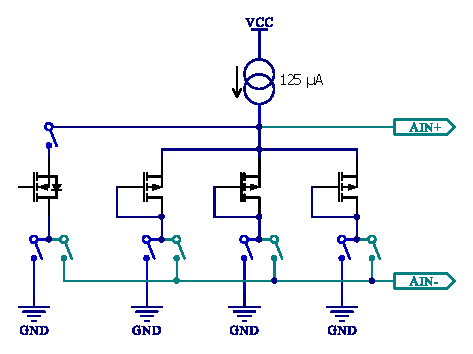
\includegraphics[width=0.7\paperwidth]{img/06/CD4007_mux_schematic.eps}
        \caption{Block diagram}
        \label{sensor_block_diagram}
    \end{figure}

\section{Low-level requirements}
    Using design requirements \ref{Design_requirements} and characteristic curves from \ref{Characteristic_curves} low-level specifications were listed:
    \begin{itemize}
        \item operating temperature range: $0 \div 60 \si{\degreeCelsius}$,
        \item compensated threshold voltage stability: \SI{\pm 0.5}{\milli\volt},
        \item current source value: $\SI{125}{\micro\ampere} \pm \SI{50}{\nano\ampere}$,
        \item ADC resolution: \SI{0.1}{\milli\volt} @ \SI{5}{\volt} reference = \SI{16}{bit}
    \end{itemize}


\section{Analog front-end}
    In this section decision and schematic diagrams of building blocks are presented.

    \subsection{SPICE models}
        Design should be validated by simulation. In this thesis, LTSpice XVII was used.

        Models used during simulation:
        \begin{itemize}
            \item CD4007 - model RIT4007P7 from Rochester Institute of Technology \cite{RIT_FULLER},
            \item Linear Technology components are embedded in LTSpice,
            \item other devices were modelled by hand using datasheets
        \end{itemize}

    \subsection{Linear regulator}
        Positive rail $+\SI{5}{V}$ on PC-104 stack comes from EPS, more specifically, this voltage is generated by DC-DC converter (with \SI{500}{\kilo\hertz} switching frequency). Because of low noise requirements analog supply voltage have to be very well regulated and filtered. Because $V_{TH}$ of transistor will increase with absorbed dose, dropout from \SI{5}{\volt} should be as low as possible. As a tradeoff between this requirement and available solutions on market analog rail voltage was chosen to be \SI{4.7}{\volt}.

        As an LDO regulator LT3042 was selected. It is ultralow noise, ultrahigh PSRR RF linear regulator by Linear Technology. Key specs \cite{LT3042_datasheet}:
        \begin{itemize}
            \item ultralow noise \SI{0.8}{\micro\volt RMS} (\SI{10}{\hertz} to \SI{100}{\kilo\hertz}),
            \item output current \SI{200}{\milli\ampere}
            \item input range \SI{1.8}{\volt} to \SI{20}{\volt}, output range \SI{0}{\volt} to \SI{15}{\volt}
            \item ultrahigh PSRR \SI{79}{\decibel} at \SI{500}{\kilo\hertz}, more detailed graph is shown in the figure \ref{LT3042_PSRR}.
            \item low dropout voltage of \SI{200}{\mV}
        \end{itemize}

        \begin{figure}[H]
            \centering
            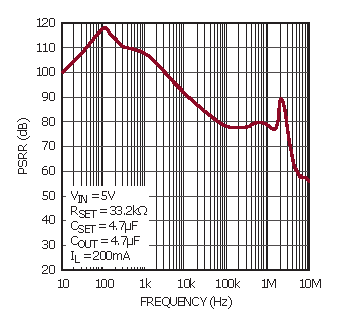
\includegraphics[width=0.4\paperwidth]{img/06/LT3042_PSRR.eps}
            \caption{LT3042 PSRR. Source: \cite{LT3042_datasheet}}
            \label{LT3042_PSRR}
        \end{figure}

        Thanks to this regulator, conducted susceptibility requirement was met (\SI{175}{\mV} input ripple is cut down to \SI{19}{\uV}, which is enough for ADC to filter).

    \subsection{RadFET power switch}
        Because main PLD microcontroller is also controlling other sensors (photodiodes, temperature sensors) RadFET analog front-end have to have a possibility to be turned off. For this purpose, TPS2551DBVx current-limited power-distribution switch was implemented in the design.

        More accurately, two of them - one to disable digital part of ADC and second to disable all analog part of the design.

        Apart from possibility of disabling RadFET they provide point-of-load latch-up current limitation, allowing to cut down power in case of SEE even faster.

    \subsection{Current source}
        Current source have to be the most accurate part of the design, because measured voltage depends in square of its variation. It was assumed that $\SI{50}{\nano\ampere}$ current stability across temperature and aging range will be sufficient. Current source have to supply both MOSFET (static resistance in operating point of about $20-25$~\si{\kilo\ohm}) and body diode temperature sensor (static resistance in operating point of about     $3-7$~\si{\kilo\ohm})

        Main concept of current source is based on Burr-Brown application note \cite{Make_a_precision_current_source_or_sink}. Idea schematic is shown in the figure \ref{current_source_schematic}.

        \begin{figure}[H]
            \centering
            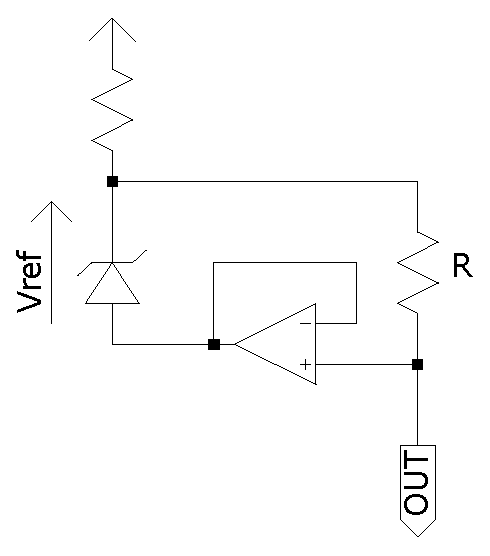
\includegraphics[width=0.3\paperwidth]{img/06/current_source_schematic.eps}
            \caption{Threshold voltage readout block diagram}
            \label{current_source_schematic}
        \end{figure}

        Output current is set by shunt voltage reference and resistor $R$, given by equation:
        $$I_{OUT} = V_{ref}/R$$

        Therefore, stability of output current depends on reference voltage and resistor accuracy.

        \bigskip \textbf{Shunt reference}

        After irradiation MOSFET $V_{DS}$ is planned to be no more than \SI{2.5}{\volt}, so reference voltage have to be lower than \SI{2}{\volt}.

        Linear Technology LT1634-1.25 shunt voltage reference was chosen. It is one of the best shunt references from Linear Technology. Basic specification:
        \begin{itemize}
            \item \SI{0.05}{\percent} initial accuracy,
            \item \SI{10}{ppm/\degreeCelsius} maximum temperature drift,
            \item $< \SI{1}{\ohm}$ dynamic resistance,
            \item \SI{10}{\uA} minimal regulation current
        \end{itemize}

        Shunt resistance was chosen to make minimal current flowing through shunt reference large enough for specified loads - final value of \SI{5}{\kilo\ohm}.

        \bigskip \textbf{Series resistor}

        Value of this resistor reflects required current flowing through MOSFET. Nominal value selected was \SI{10}{\kilo\ohm}.

        Stability of this resistor across temperature is critical because it directly changes output current. To achieve specified requirement \SI{10}{\kilo\ohm} / \SI{5}{ppm} resistor was chosen (APC0603T10K0Z).

        Manufacturer does not specify exact value and profile of the temperature coefficient - so both worst cases was simulated (\SI{-5}{ppm} and \SI{5}{ppm}).

        \bigskip \textbf{Operational amplifier}

        Operational amplifier in this circuit should have very low bandwidth (noise limitation), low offset voltage (precision) and small footprint. LTC2054 was selected - key characteristics:
        \begin{itemize}
            \item \SI{3}{\micro\volt} offset voltage,
            \item common mode $\pm \SI{0.5}{\volt}$ input/output range,
            \item \SI{500}{\kilo\hertz} gain-bandwidth product,
            \item device in Military Plastic package (temperature range $-55 \div \SI{150}{\degreeCelsius}$)
        \end{itemize}

        \bigskip \textbf{Simulation}
        Behavioral simulations were performed to found all possible problems with circuit:
        \begin{itemize}
            \item temperature dependency,
            \item output resistance range,
            \item noise and stability
        \end{itemize}

        MOSFET/diode was replaced by resistor emulating its static resistance ($\SI{2}{\volt}/\SI{125}{\micro\ampere} = \SI{16}{\kilo\ohm}$, $\SI{0.6}{\volt}/\SI{125}{\micro\ampere} = \SI{5}{\kilo\ohm}$, respectively). Simulation view is shown in the figure \ref{current_source_simulation}.

        \begin{figure}[H]
            \centering
            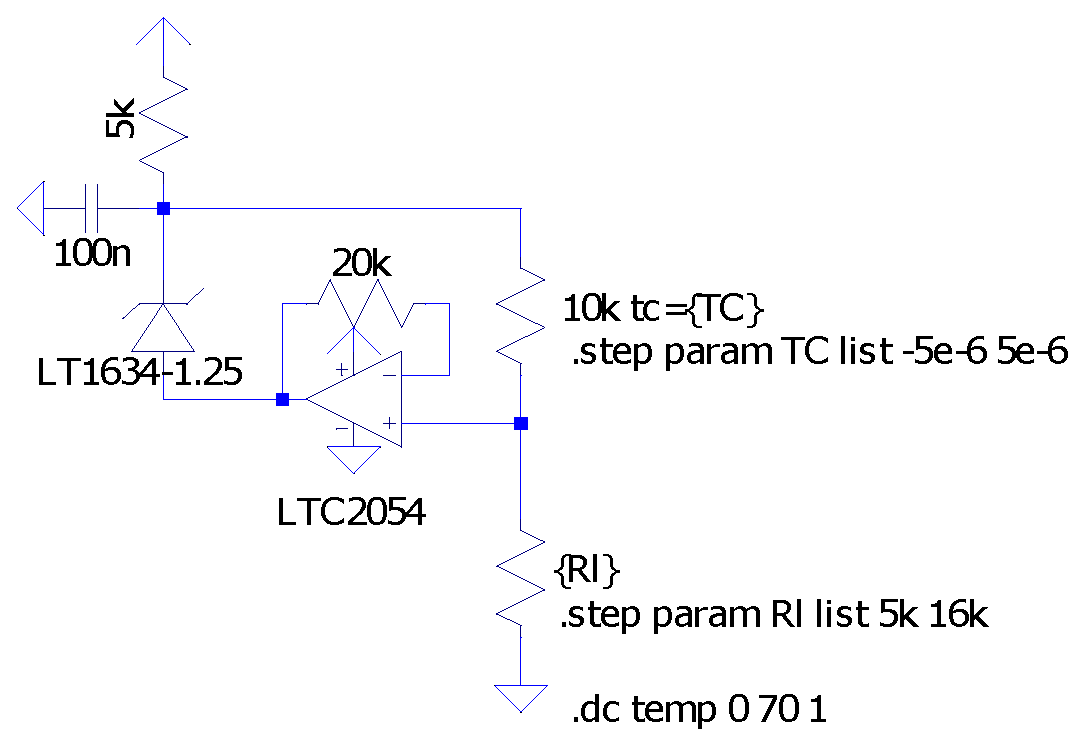
\includegraphics[width=0.5\paperwidth]{img/06/current_source.eps}
            \caption{Current source simulation}
            \label{current_source_simulation}
        \end{figure}

        \bigskip\textbf{Temperature dependency}
        Output current is shown in the figure \ref{current_source_simulation_result}, simulation was performed on two different loads and resistor temperature coefficients.
        \begin{figure}[H]
            \centering
            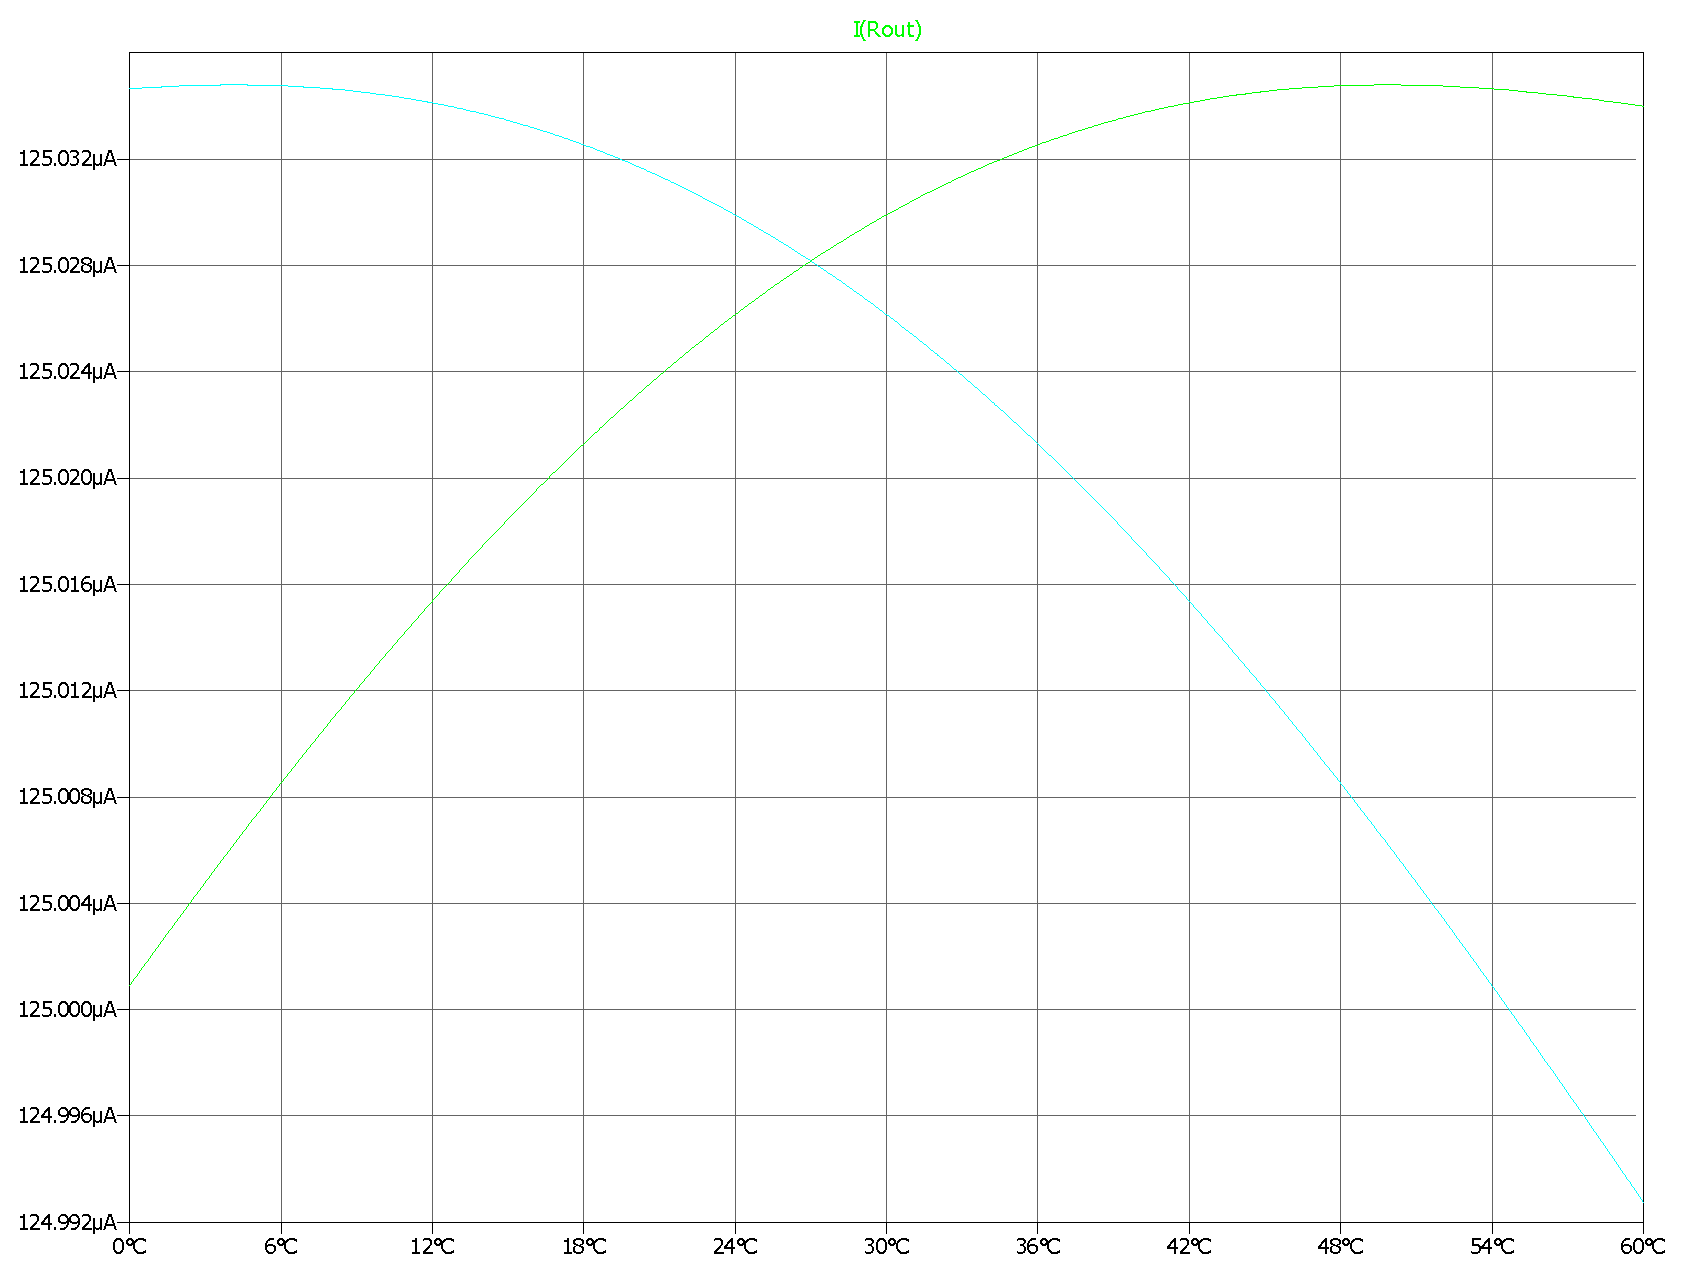
\includegraphics[width=0.8\paperwidth]{img/06/current_source_result.eps}
            \caption{Current source simulation result - output current}
            \label{current_source_simulation_result}
        \end{figure}

        In both cases current change across temperature range does not exceed \SI{40}{\nano\ampere}.

        \bigskip\textbf{Output resistance range}
        \bigskip\textbf{Noise density}
        \bigskip\textbf{Stability}

    \subsection{Analog to digital converter}
        Analog to digital converter is responsible for reading $V_{DS}$ voltage across transistor and voltage across diode. Due to very low changes, high accuracy and resolution is required. Additionally, complex mixed signal element like ADC should have radiation tests to prove its long term reliability. To achieve at least \SI{0.1}{\milli\volt} resolution ADC has to be at least \SI{16}{bits}.

        Due to constrain on system and reliability the AD7714 from Analog Devices was chosen. Radiation tests shown that it fails between \SI{10}{\kilo\rad} and \SI{20}{\kilo\rad}, with no degradation up to \SI{10}{\kilo\rad} \cite{ADC_radiation_tests}.

        Internal diagram can be found in the figure \ref{AD7714}. Key specs:
        \begin{itemize}
            \item \SI{24}{bits},
            \item \SI{0.0015}{\percent} nonlinearity,
            \item programmable gain ($1 \div 128$),
            \item 3 fully differential or 5 pseudo-differential input channels
            \item \SI{3}{\volt} or \SI{5}{\volt} operation
            \item separated digital and analog supply and grounds,
            \item SPI interface
            \item \SI{0.25}{\hertz} sampling frequency for strongest filter,
        \end{itemize}

        \begin{figure}[H]
            \centering
            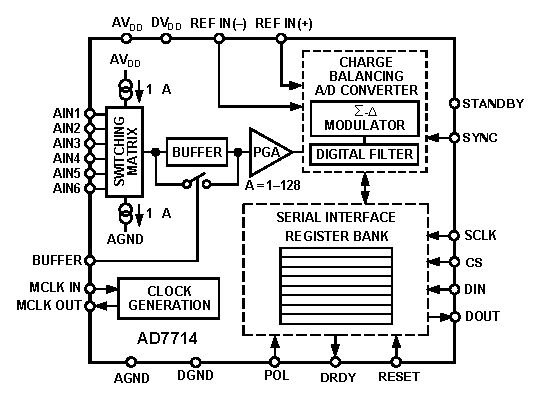
\includegraphics[width=0.5\paperwidth]{img/06/AD7714.eps}
            \caption{AD7714 internal block diagram. Source: \cite{AD7714_datasheet}}
            \label{AD7714}
        \end{figure}

        AD7714 requires external crystal or clock oscillator in frequency range \SI{1}{\mega\hertz} to \SI{2.54}{\mega\hertz}. Crystal oscillators for these frequencies are large and susceptible for shocks and damages because of large, delicate internal structure. \SI{1}{\mega\hertz} ceramic oscillator ISM95-3351AH was selected for operation. Comparison of solution in shown in the figure \ref{crystal_oscillator_difference}.

        \begin{figure}[H]
            \centering
            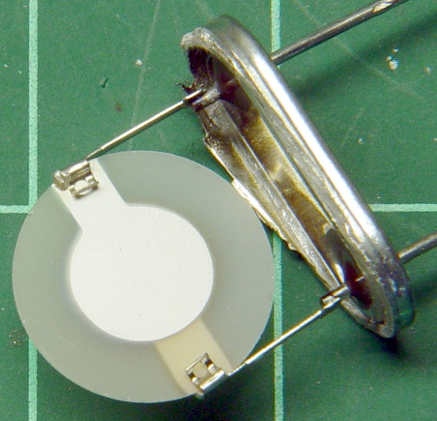
\includegraphics[width=0.35\paperwidth]{img/06/crystal.png}
                        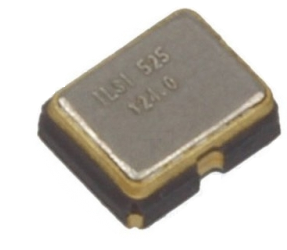
\includegraphics[width=0.35\paperwidth]{img/06/ISM95.png}
            \caption{Low frequency crystal oscillator internals. Source: \cite{Opening_a_Quartz_Crystal_Can_Effects_Thereof}, ISM95-3351AH-1.0000 ceramic oscillator package. Source: \cite{ISM95_series_datasheet}}
            \label{crystal_oscillator_difference}
        \end{figure}

    \subsection{Multiplexer}
        Multiplexer have two purposes: to multiplex current and voltage lines (3-wire readout).

        As an analog multiplexer ADG709 was chosen. Its radiation tests can be found in \cite{IEEE_radiation_tests_1992_2009}. It is double 1:4 mux, allowing simultaneous current and voltage multiplexing. Internal block diagram is shown in the figure \ref{ADG709_block}

        \begin{figure}[H]
            \centering
            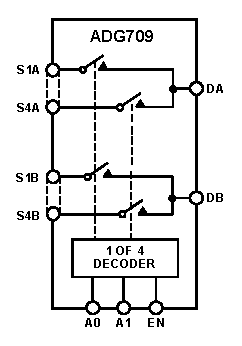
\includegraphics[width=0.3\paperwidth]{img/06/ADG709.eps}
            \caption{ADG709 internal block diagram. Source: \cite{ADG709_datasheet}}
            \label{ADG709_block}
        \end{figure}

        Due to ESD diodes id CD4007 additional current switch had to be added to cut off potential from from n-MOS body diode. For this purpose simple 1-channel analog switch ADG849YKSZ was implemented.

    \subsection{Differential \& common mode filter}
        Internal sampling frequency of ADC (for GAIN = 1 and $f_{clk} = \SI{1}{\mega\hertz})$ is about \SI{15.6}{\kilo\hertz}. To eliminate aliasing and reduce readout noise low-pass differential filter should be implemented on ADC input.

        Simple one-pole RC filter was selected. Its schematic can be found in the figure \ref{low_pass_filter}.

        \begin{figure}[H]
            \centering
            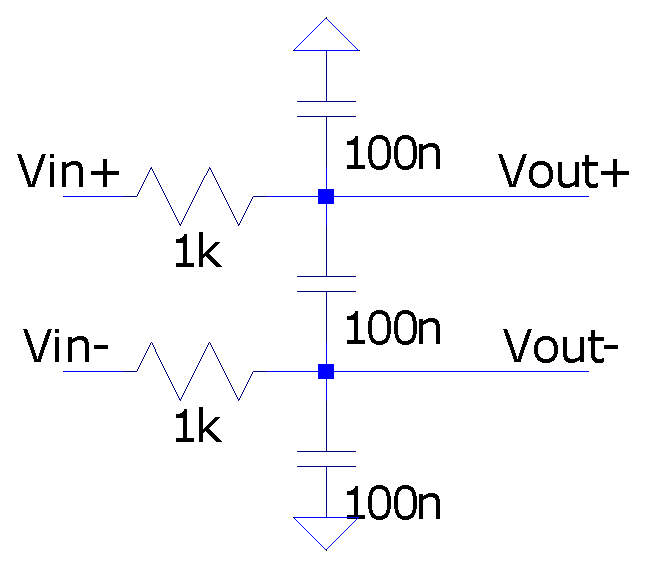
\includegraphics[width=0.3\paperwidth]{img/06/low_pass_filter.eps}
            \caption{Low pass filter schematic.}
            \label{low_pass_filter}
        \end{figure}

        Using AC analysis its frequency characteristic was obtained - figure \ref{low_pass_filter_output}. At half of sampling frequency attenuation is about \SI{22}{\decibel}.

        \begin{figure}[H]
            \centering
            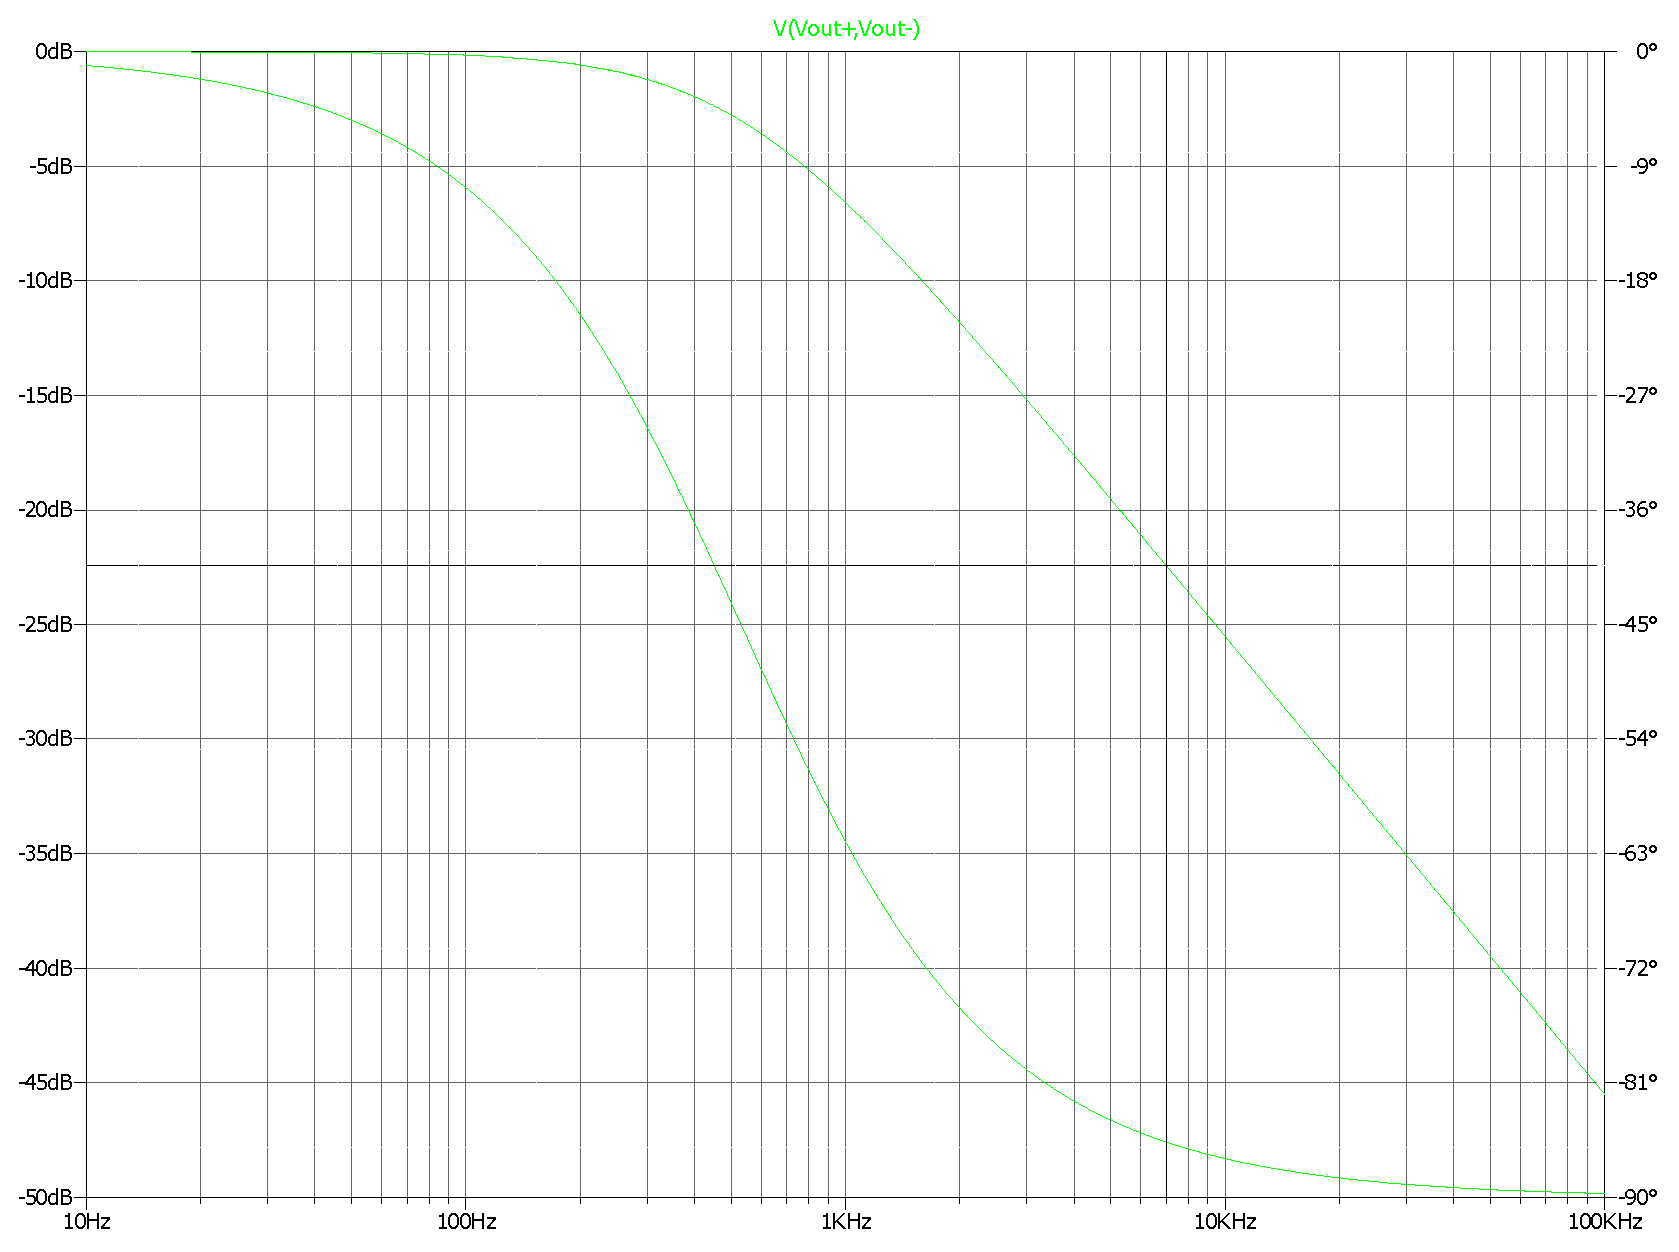
\includegraphics[width=0.6\paperwidth]{img/06/low_pass_filter_output.eps}
            \caption{Low pass filter frequency characteristics.}
            \label{low_pass_filter_output}
        \end{figure}

    \subsection{Shielding}
        Because of noise requirements and near proximity of \SI{0.5}{\watt} radio transmitter, EMI shielding was tested.

        Proper pads for EMI shielding were placed on PCB. Its size depends on PCB layout, after routing it was decided to use BMI-S-203 shield (figure \ref{BMI-S-203}). This shield should provide attenuation of about \SI{50}{\decibel} on transmitter frequency.

        \begin{figure}[H]
            \centering
            
\includegraphics[width=0.7\paperwidth]{img/06/BMI-S-203.eps}
            \caption{BMI-S-203 shield. Source: \cite{EMI_shieldings_catalog}}
            \label{BMI-S-203}
        \end{figure}


\section{Digital}
    RadFET is mainly analog sensor. But, LDO, MUX and ADC has to be controlled from on-board microcontroller. On other hand, RadFET have to be accessible from OBC, to retrieve data and send them to the ground station.

    \subsection{Microcontroller}
        Main digital part of the design is microcontroller. It will be responsible for:
        \begin{itemize}
            \item controlling analog part of the sensor,
            \item implementing FDIR in case of any failure,
            \item communicating with OBC to retrieve data.
        \end{itemize}

        Couple of options were considered, and the final choose was ATmega164PV-10AQ. More detailed comparison can be found in \cite{PWSAT_EPS_CDR}.

        AVR devices are known from their simplicity, reliability and very little bugs. Radiation tests were performed for ATmega series, showing their performance for up to \SI{14}{\kilo\rad} \cite{ATMEGA128_radiation_tests}.

        Features of this particular device:
        \begin{itemize}
            \item \SI{1.8}{\volt} - \SI{5.5}{\volt} supply voltage,
            \item \SI{4}{\mega\hertz} clock,
            \item TQFP-44 package,
            \item \SI{16}{\kilo B} program memory,
            \item \SI{1}{\kilo B} SRAM
        \end{itemize}

    \subsection{On-Board Computer interface}
        Interface to OBC is $I^2C$ bus. Because sensor can be turned off by cutting its voltage proper buffering had to be implemented. For this purpose $I^2C$ repeater PCA9517 was placed between OBC and in-sensor microcontroller. Its functional diagram can be seen in the figure \ref{PCA9517}. From its datasheet: "The SDA and SCL pins are over voltage tolerant and are high-impedance when the PCA9517 is unpowered." \cite{PCA9517_datasheet}. Thanks to it OBC can completely disable the sensor, by simply cutting it a power.

        \begin{figure}[H]
            \centering
            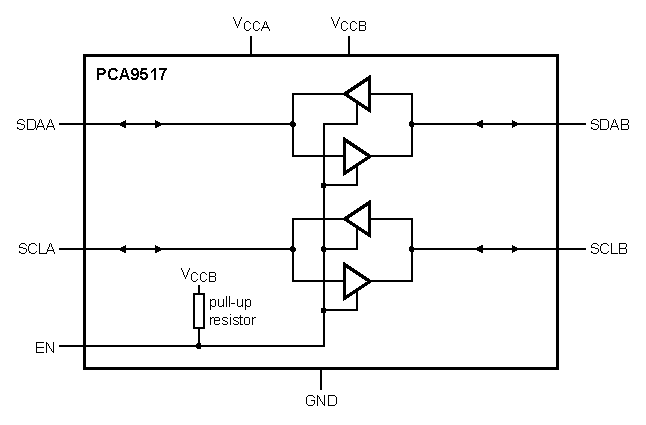
\includegraphics[width=0.7\paperwidth]{img/06/PCA9517.eps}
            \caption{PCA9517 internal block diagram. Source: \cite{PCA9517_datasheet}}
            \label{PCA9517}
        \end{figure}


\section{Final schematic}
    Top level schematic file can be seen in the figure \ref{top_level_schematic}. Ports represents physical connectors - to satellite bus and debug socket.

    \begin{figure}[H]
        \centering
        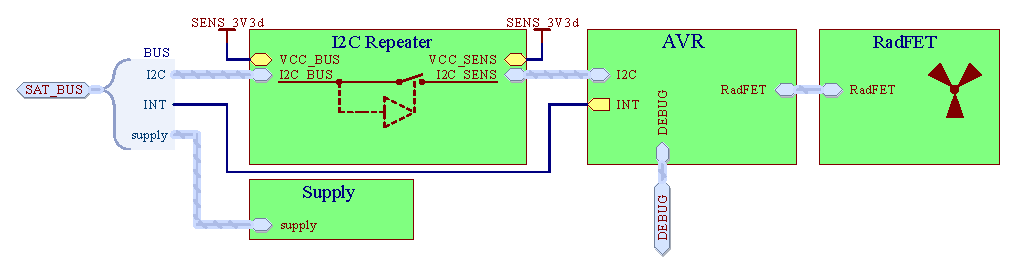
\includegraphics[width=0.8\paperwidth]{img/06/final_schematic_top.eps}
        \caption{Top level schematic}
        \label{top_level_schematic}
    \end{figure}

    "RadFET" consists analog part of the design. Its block diagram can be seen in the figure \ref{analog_schematic}.

    \begin{figure}[H]
        \centering
        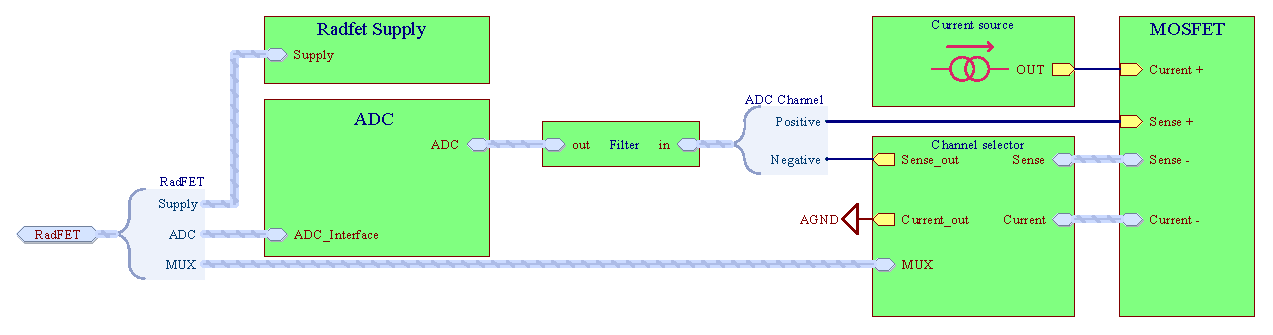
\includegraphics[width=0.8\paperwidth]{img/06/final_schematic_radfet.eps}
        \caption{Sensor final schematic - analog part}
        \label{analog_schematic}
    \end{figure}


\section{PCB}
    Engineering model of the sensor was manufactured on similar board to the flight model. It should represent space required for this sensor, noise coupling and performance.

    For schematic capture, PCB layout \& DRC Altium Designer EDA software was used.

    \subsection{PCB materials}
        During initial phase of PW-Sat2 project it was decided that all self-made board will be manufactured on FR4 laminate. Despite most space-qualified PCBs are made of polimide, it will be very hard (and expensive) to manufacture them. Despite higher glass transition temperature they do not provide much advantages.

        But, careful should be taken to check for:
        \begin{itemize}
            \item vibration tolerance,
            \item gluing quality of multiple layer boards,
            \item outgassing coefficient.
        \end{itemize}

        Having this in mind manufacturer of PCB was selected - Technoservice S.A.

    \subsection{PCB stack}
        Because outgassing of devices can be dangerous for turbomolecular pumps, it have to be limited as much as possible. Therefore soldermask and overlay layers are not present in the design, and packages of used components have known outgassing coefficients.

        For this prototype board have 4 layers, on flight model board will be 6-layered. PCB stack generated from Altium Designer is shown in the figure \ref{PCB_Altium_stack}.

        \begin{figure}[H]
            \centering
            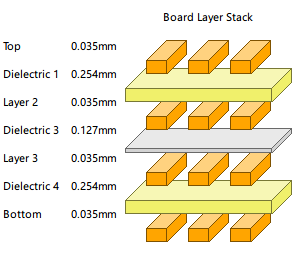
\includegraphics[width=0.3\paperwidth]{img/06/stack.png}
            \caption{Sensor PCB stack}
            \label{PCB_Altium_stack}
        \end{figure}

    \subsection{PCB layout}
        PCB layout in mixed signal board is very important. Ground potential shifts, induced noise, coupling between ground planes - all those effects were considered during layout process.

        \bigskip \textbf{Top \& bottom layers}

        On top and bottom layers only components should be placed, every net should be connected on internal layers. But, because of having only 4-layer board this design recommendation is not fulfilled - this will be forced on Flight Model. Final layout is shown in the figure \ref{top_bottom_layer_layout}.

        \begin{figure}[H]
            \centering
            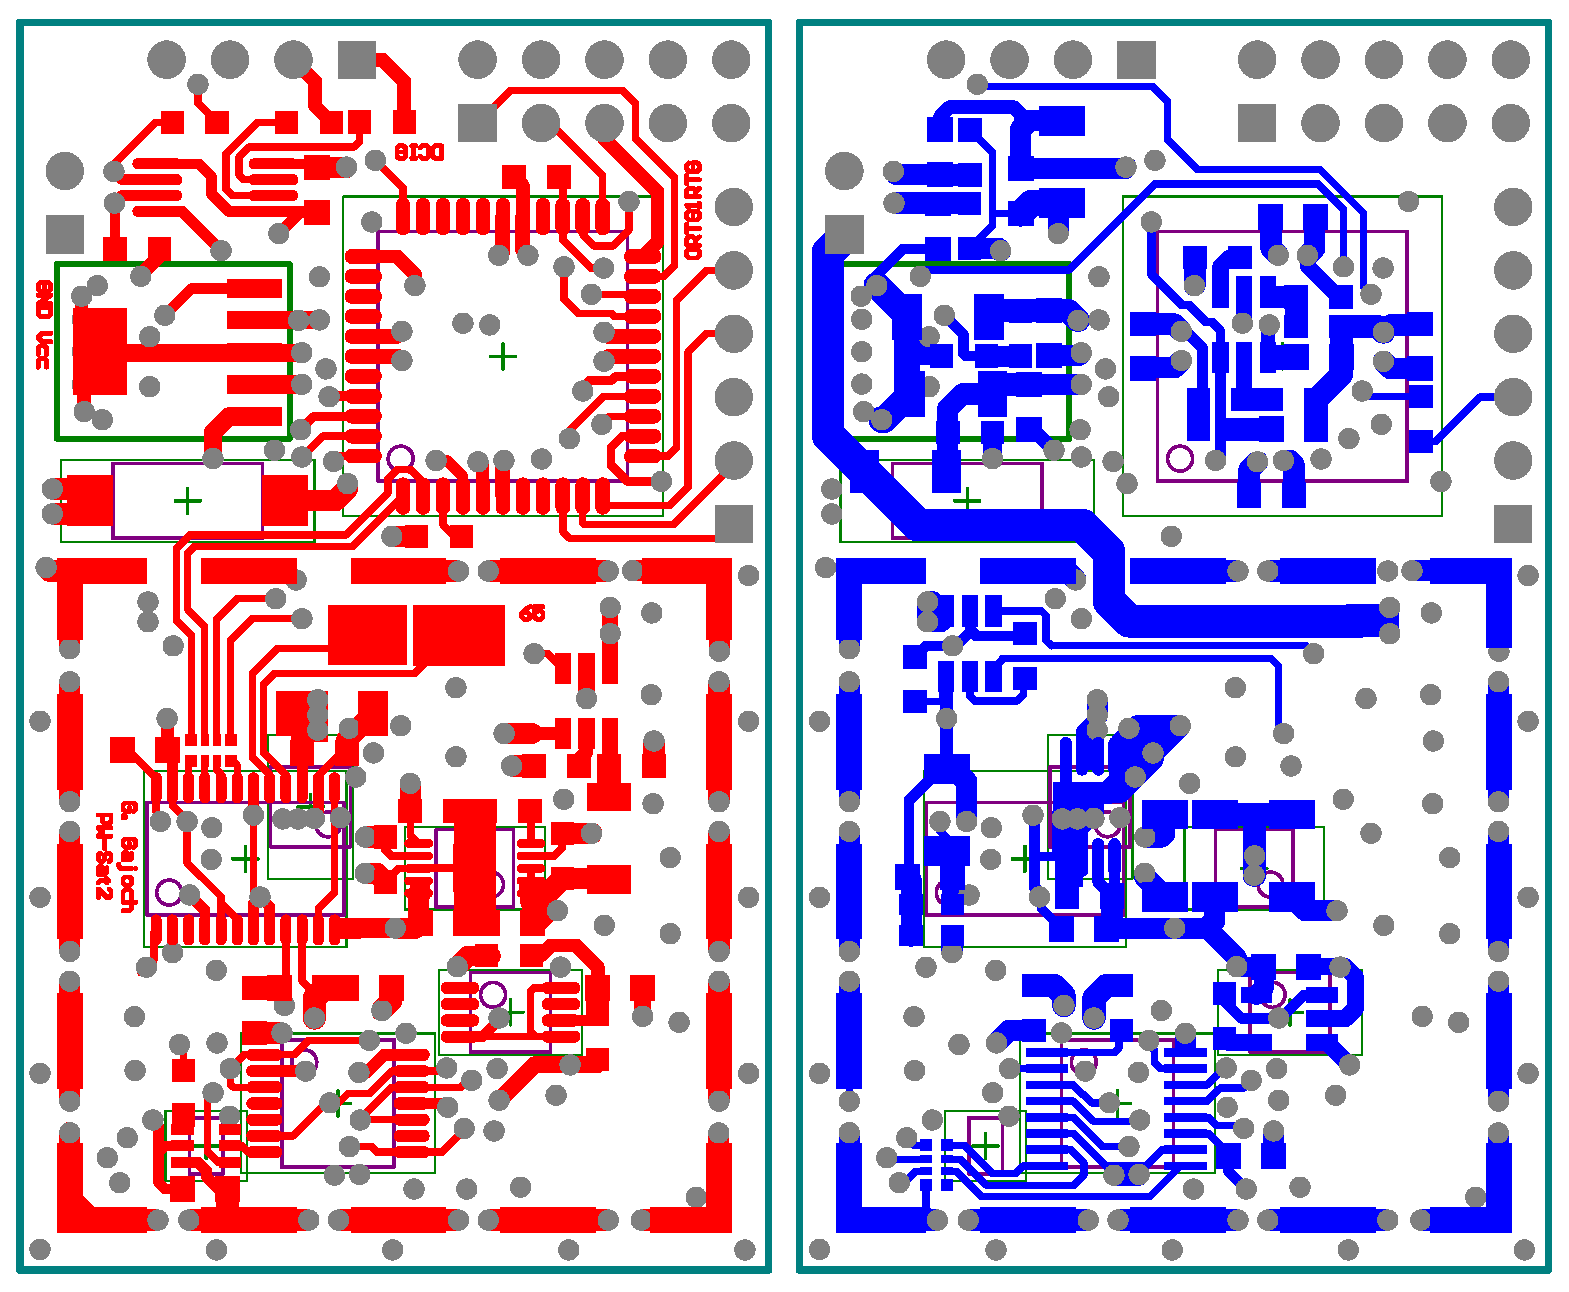
\includegraphics[width=0.5\paperwidth]{img/06/top_bottom_layer_layout.eps}
            \caption{Top and bottom layer layout}
            \label{top_bottom_layer_layout}
        \end{figure}

        \bigskip \textbf{Internal layers}

        One layer of board was designed to be completely a ground plane. More specifically, two ground planes - analog and digital one, connected under ADC. Second internal layer provides routing space, but also have ground planes on it (due to PCB temperature bending PCB cannot have only one ground plane). Layout is shown in the figure \ref{internal_layers_layout}.

        \begin{figure}[H]
            \centering
            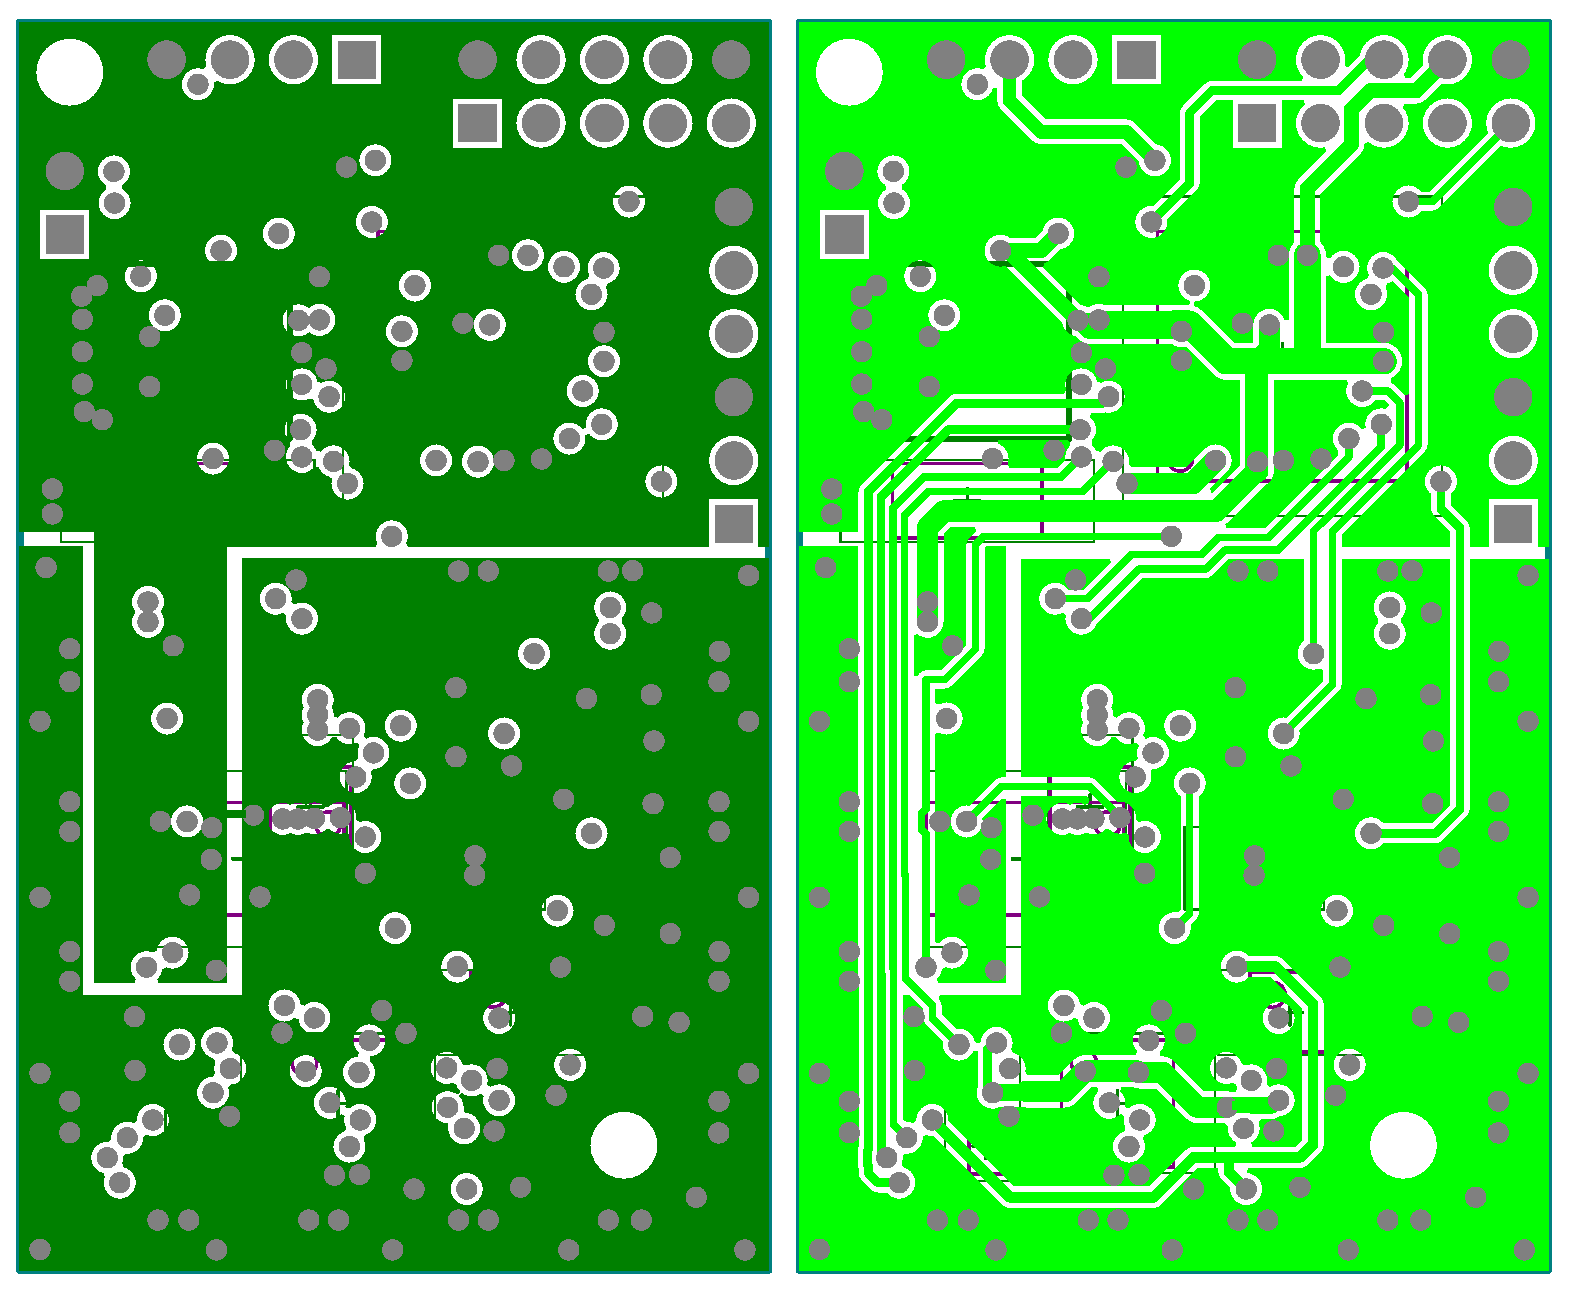
\includegraphics[width=0.5\paperwidth]{img/06/internal_layers_layout.eps}
            \caption{Internal layers layout}
            \label{internal_layers_layout}
        \end{figure}

    \subsection{3D model}
        Using Altium designer and proper self-made libraries, 3D model of board can be easily generated. In the figure \ref{pcb_3d_model} 3D model with and without EMI shielding is shown.

        \begin{figure}[H]
            \centering
            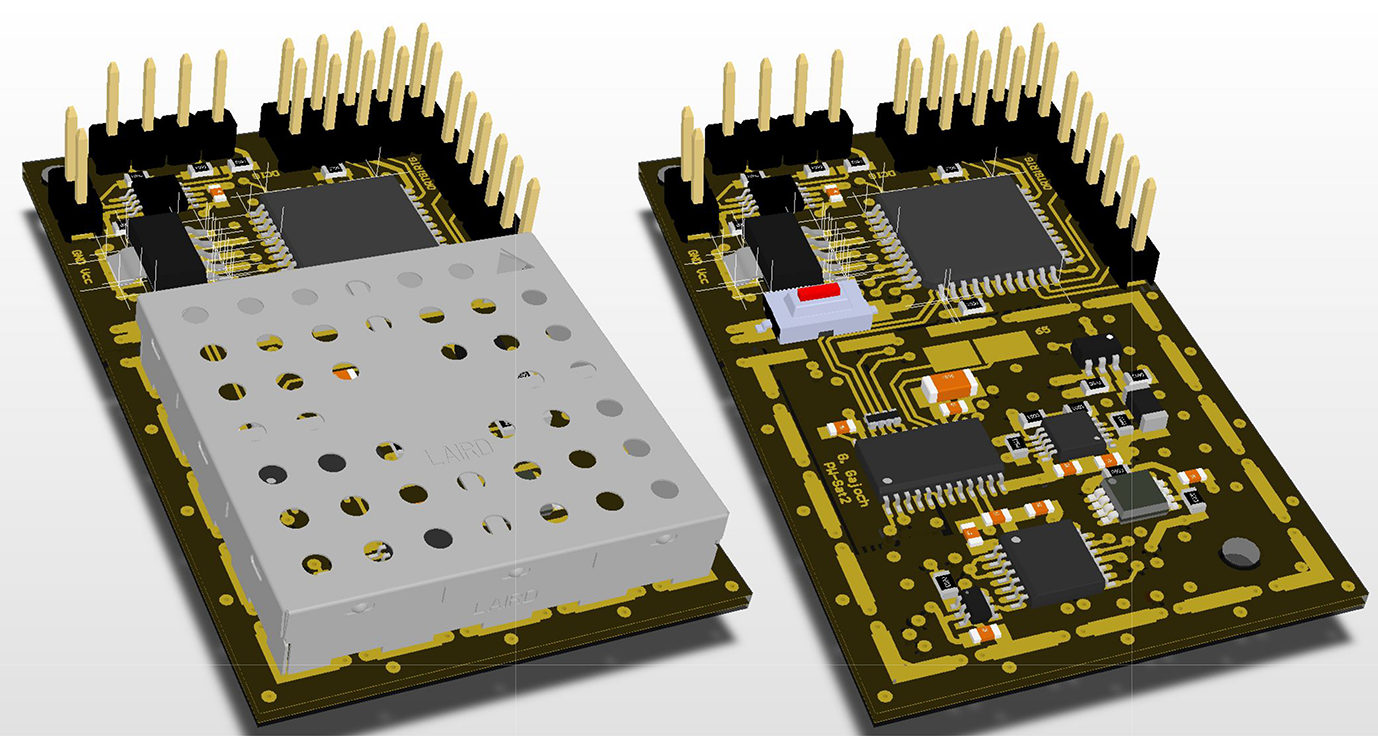
\includegraphics[width=0.8\paperwidth]{img/06/pcb_3d_model.png}
            \caption{3D view of engineering model with and without EMI shield}
            \label{pcb_3d_model}
        \end{figure}

\section{Software design}
    Important aspect of the sensor is embedded software. It has to control data acquisition (LDO, ADC, MUX), check for validity and expose \iic interface to OBC.

    Because main microcontroller is 8-bit AVR-core processor, software have to be highly optimized, especially for speed and data memory consumption. Available resources:
    \begin{itemize}
        \item \SI{16}{\kilo B} of FLASH,
        \item \SI{1}{\kilo B} of SRAM,
        \item \SI{1}{\mega\hertz} clock frequency.
    \end{itemize}

    Software for sensor was written in C++14, using developed by PW-Sat2 team AVR-HAL library. Schematic of software building blocks is shown in the figure \ref{Sensor_software_diagram}.

    \begin{figure}[H]
        \centering
        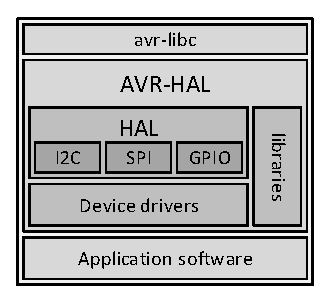
\includegraphics[width=0.5\paperwidth]{img/06/software_diagram.eps}
        \caption{Sensor software diagram}
        \label{Sensor_software_diagram}
    \end{figure}

    \subsection{AVR-HAL}
    AVR-HAL is a library created to ease software development on AVR microcontrollers. It was created by PW-Sat2 team, having in mind low overhead (in most modules zero-data usage), extensibility and modern software development languages and techniques (C++14, unit and integration testing). It was created for specific purpose which is embedded software development on-board PW-Sat modules (EPS, PLD, SunS). Therefore only few devices are officially supported (ATmega164, 165, 328), with extensible tests on existing platforms.

    AVR-HAL consists of basic modules:
    \begin{itemize}
        \item C++14 libraries not existing in avr-libc (type traits, array, array\_view),
        \item Hardware Abstraction Layer - identical low-level API for every ported device,
        \item Device Drivers - drivers for many used integrated circuits used on PW-Sat2,
        \item Debugging libraries - software created to allow unified debugging of many devices (serial port, command line interface, gdb connection etc).
    \end{itemize}

    Using AVR-HAL writing application software is only high-level work, leaving all hardware access to tested and proven library.

    \subsection{$I^2C$-slave interface}
    Cubesat standard define two \iic lines along satellite board stack, which most of the commercially available devices use. It was the easiest option for connecting PLD board to OBC, so this communication bus was selected.

    The sensor acts as a slave on \iic bus. Communication protocol is based on request-reply manner, with interrupt pin acting as a notification.

    When OBC wants to gather data from sensor it will do following tasks in order:
    \begin{itemize}
        \item send measurement start request to sensor (table \ref{Start_measurement_command}),
        \item wait until conversion is completed (pulse on interrupt line is triggered),
        \item read data from sensor internal memory (table \ref{Data_readout_command}).
    \end{itemize}

    \begin{table}[H]
        \begin{center}
            \begin{tabular}{|c|c|c|c|}
                \hline
                START & 0x20+W & 0x80 & STOP \\ \hline
            \end{tabular}
        \end{center}
        \caption{Start measurement command}
        \label{Start_measurement_command}
    \end{table}

    \begin{table}[H]
        \begin{center}
            \begin{tabular}{|c|c|c|c|c|c|c|}
                \hline
                START & 0x20+W & 0x00 & REP-START & 0x20+R & (...data...) & STOP \\ \hline
            \end{tabular}
        \end{center}
        \caption{Data readout command}
        \label{Data_readout_command}
    \end{table}

    \subsection{Measurement algorithm}
    \bigskip \textbf{RadFET sensor}

    Sensor after receiving "start measurement" command (table \ref{Start_measurement_command}) does following steps:
    \begin{itemize}
        \item enable LDO,
        \item wait for power line stabilization,
        \item for each channel in [MOS0, MOS1, MOS2, TEMPERATURE]:
        \begin{itemize}
            \item[$\circ$] select proper MUX switch,
            \item[$\circ$] enable MUX,
            \item[$\circ$] wait for stabilization,
            \item[$\circ$] read ADC value,
            \item[$\circ$] disable MUX
        \end{itemize}
        \item disable LDO,
        \item make a positive pulse on interrupt line, informing OBC about conversion finish.
    \end{itemize}

    \bigskip \textbf{OBC}

    When OBC wants to read data form sensor (issued by telecommand from ground station) it perform following steps:
    \begin{itemize}
        \item enable PLD power by sending proper command to EPS,
        \item send "start measurement" command to RadFET,
        \item wait for trigger on interrupt line (external interrupt pin),
        \item send "data readout" command and store data in memory,
        \item disable power for PLD board
    \end{itemize}

\section{Assembly}
    For final model, proper ECSS standards will be applied during soldering and integration. On engineering model proper tools and techniques should be tested to eliminate unnecessary problems later on.

    Equipment used during soldering and integration are compliant with ECSS standards, same tools would be used on flight hardware:
    \begin{itemize}
        \item Weller WMRP station,
        \item \SI{63}{\percent} Sn/\SI{37}{\percent} Pb \SI{0.2}{\milli\meter} soldering wire,
        \item Alpha RMA - ROL0 flux,
        \item ESD-protected workstation and tools.
    \end{itemize}

\section{Finished sensor}
    Photo of sensor after integration can be seen in the figure \ref{Integrated_sensor}.

    \begin{figure}[H]
        \centering
        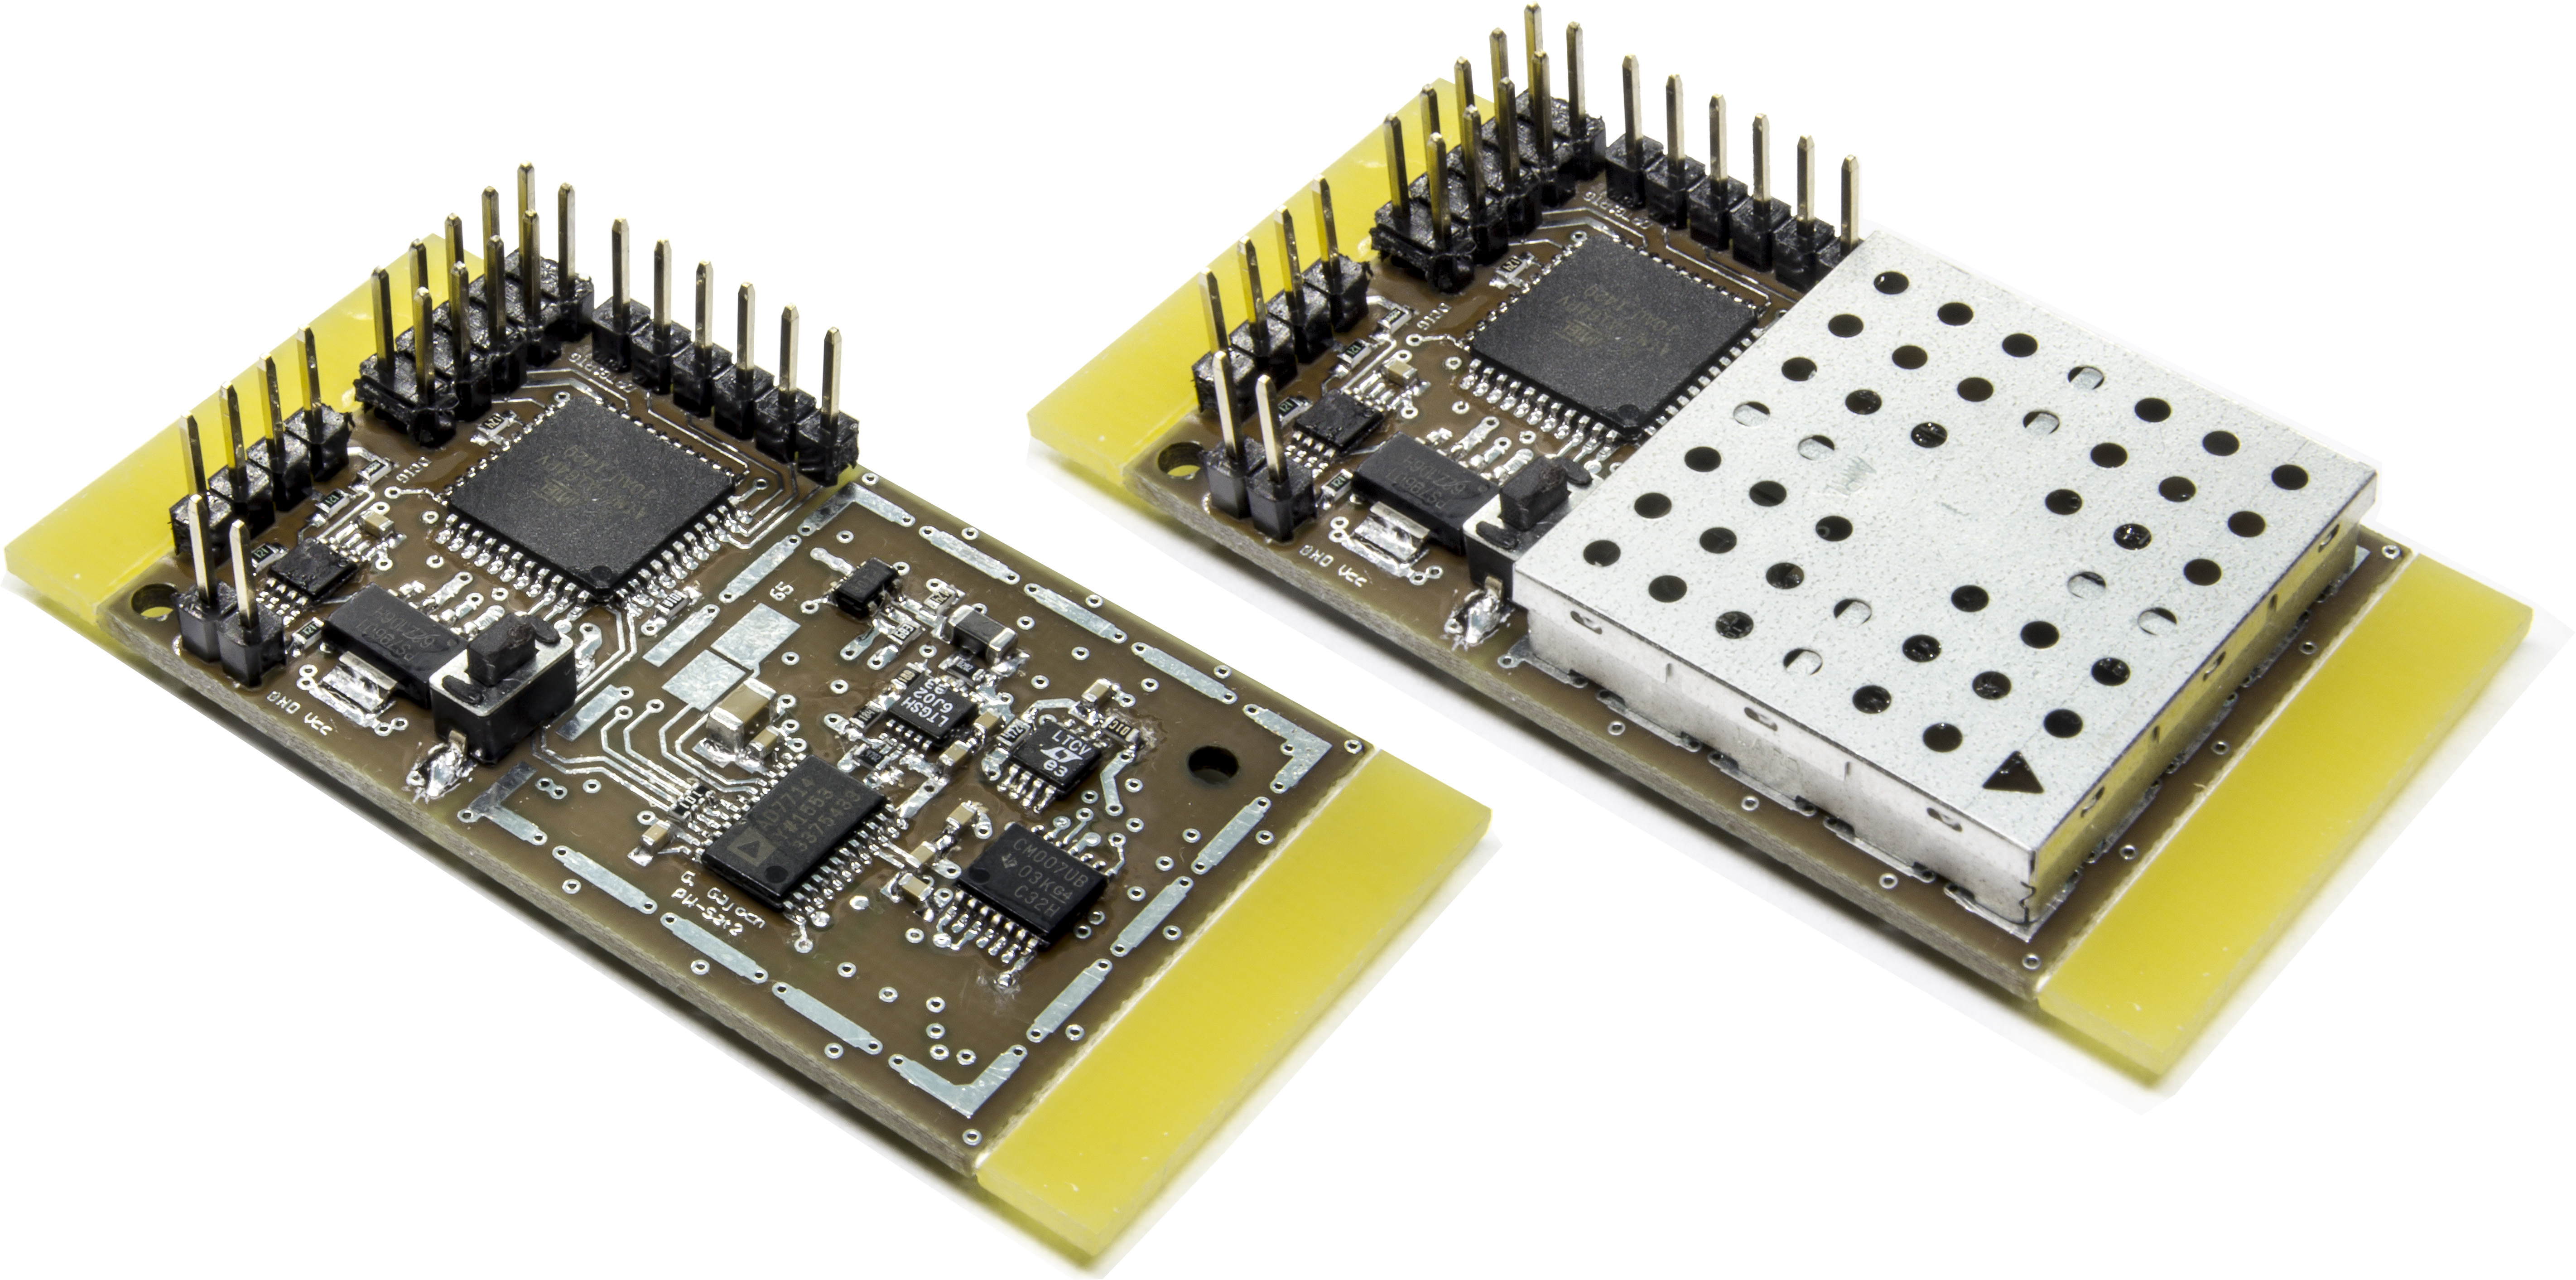
\includegraphics[width=0.8\paperwidth]{img/06/finishiedSensorPhoto.jpg}
        \caption{Integrated sensor without and with EMI shield}
        \label{Integrated_sensor}
    \end{figure}
